\section{Results in two dimensions}\label{sec:results2d}

The two-dimensional comparison is the pre-registered run of 9 October 2026, made with the
later code of \cref{sec:methods:networks}, which multiplies the decoded field by $F_{\max}$
as in three dimensions. It trained again two networks of an earlier pre-registered run,
that of 16 July 2026, on the same corpus, split and seeds and with the same training
settings: the supervised transformer, with every number of labelled instances, and the
graph network, with 64 and 1,024 only (\cref{sec:methods:training}). Beside them it
evaluated, without retraining them, the three label-free transformers that the run of 29
September 2026 had trained with the same code on the same 1,024 instances (the
unregularised networks of \ref{app:e1}). It added one network, the stiffness-norm
transformer: the supervised transformer trained on the relative stiffness-norm error
\eqref{eq:lk} instead of the relative displacement error \eqref{eq:ld}, with the same
labels, which separates the norm of the loss from the labels (\cref{sec:results2d:norm}).
The trained networks of this section are thus the label-free, the supervised and the
stiffness-norm transformers and the graph network. The run of 16 July 2026 is reported in
\cref{sec:results2d:july}; the configuration hashes of both runs are given in
\ref{app:repro}.

\subsection{Accuracy}\label{sec:results2d:accuracy}

% generated by scripts/make_cmame_material.py from the records; do not edit
\begin{table}[tbp]
\centering
\footnotesize
\setlength{\tabcolsep}{4pt}
\caption{Two-dimensional plates, every metric at the largest label budget. The supervised networks were trained on 1,024 labelled instances; the label-free network on the same 1,024 instances without their solutions.}
\label{tab:2d}
\resizebox{\ifdim\width>\textwidth\textwidth\else\width\fi}{!}{%
\begin{tabular}{lcccccc}
\toprule
Model & \shortstack{Displacement \\ error} & \shortstack{Relative \\ energy gap} & \shortstack{von Mises \\ error} & \shortstack{Peak stress \\ error} & \shortstack{Critical-region \\ recall} & \shortstack{Worse than \\ zero field} \\
\midrule
Label-free & 0.166 $\pm$ 0.002 & 0.0817 $\pm$ 0.0040 & 0.210 $\pm$ 0.003 & 0.228 $\pm$ 0.001 & 0.739 $\pm$ 0.003 & 3/768 \\
Supervised & 0.160 $\pm$ 0.003 & 0.418 $\pm$ 0.037 & 0.433 $\pm$ 0.031 & 0.334 $\pm$ 0.036 & 0.584 $\pm$ 0.027 & 52/768 \\
Supervised + energy term & 0.161 $\pm$ 0.005 & 0.166 $\pm$ 0.040 & 0.257 $\pm$ 0.007 & 0.246 $\pm$ 0.022 & 0.708 $\pm$ 0.012 & 14/768 \\
Label-free, then supervised & 0.166 $\pm$ 0.006 & 0.236 $\pm$ 0.032 & 0.336 $\pm$ 0.020 & 0.301 $\pm$ 0.019 & 0.645 $\pm$ 0.008 & 21/768 \\
Graph network, supervised & 0.167 $\pm$ 0.000 & 2.57 $\pm$ 0.25 & 1.10 $\pm$ 0.07 & 1.32 $\pm$ 0.13 & 0.322 $\pm$ 0.027 & 481/768 \\
\midrule
Nearest-neighbour field & 0.404 & 0.959 & 0.735 & 0.643 & 0.515 & 94/256 \\
Scaled polynomial & 1.42 & 873 & 11.4 & 30.8 & 0.159 & 256/256 \\
\midrule
Zero field & 1.00 & 1.00 & 1.00 & 1.00 & -- & -- \\
\bottomrule
\end{tabular}}

\smallskip
\begin{minipage}{\linewidth}\footnotesize\raggedright
256 validation instances, never trained on; four load cases each. Errors are relative to the reference finite-element solution, per load case, then averaged over the load cases; the relative energy gap of the zero field is 1. Trained networks: mean $\pm$ sample standard deviation over 3 seeds; the nearest-neighbour field and the scaled polynomial are deterministic.\par
Worse than zero field: instance-seed pairs whose relative energy gap exceeds 1, that is, predictions further from the solution in the energy norm than the zero field.\par
Critical-region recall: the share of the 10\% most stressed elements of the reference solution that are also among the 10\% most stressed of the prediction (higher is better; in every other column lower is better).\par
Run of 16 July 2026. Its code did not multiply the load scale back onto the output (\cref{sec:methods:networks}); we attribute the narrow spread of the displacement errors to this, untested (\cref{sec:results2d:other}).
\end{minipage}
\end{table}


\Cref{tab:2d} gives every metric with 1,024 labelled instances. The label-free transformer
was more accurate than the supervised transformer, the same network trained on the solutions
of the same instances, on every metric but the displacement error, in each of the three
seeds: its relative energy gap, \numCmFreeGap{}, was \numCmLabOverFreeGap{} times lower, and
its von Mises error (\numCmFreeVm{} against \numCmLabVm{}), peak stress error
(\numCmFreePeak{} against \numCmLabPeak{}) and critical-region recall (\numCmFreeRecall{}
against \numCmLabRecall{}) were better. Its displacement error, \numCmFreeDispFour{}, was
\numCmFreeDispExcessAbs{} higher than the supervised transformer's, \numCmLabDispFour{}, and
higher in each seed, by \numCmFreeDispExcessMin{} to \numCmFreeDispExcessMax{}. Compared
instance by instance within each seed, the label-free transformer had the lower relative
energy gap on \numPairCmLabGap{} of the \numCmPairs{} instance-seed pairs and the lower von
Mises error on \numPairCmLabVm{}, but the lower displacement error on only
\numPairCmLabDisp{}; on \numPairCmOpposite{} of the pairs the displacement error and the von
Mises error ranked the two networks in opposite orders (\cref{rem:rank}).

The pre-registered hypothesis H1, that the label-free transformer has the lower relative
energy gap, was supported: its seed mean was \numHOneRel{} lower, beyond the noise guard of
\numHOneTau{}. The guard, fixed in the pre-registration, is the larger of 10\% and twice the
standard error of the relative difference of the two seed means (note to
\cref{tab:criteria}); a difference within it is reported as no difference shown, which is
not equivalence. \Cref{tab:cm2d} gives, for H1 and the other hypotheses of this run, the
per-seed values and the readings that the pre-registration required beside each verdict:
on the seeds' medians over the instances the guard gave the same readings, and the 95\%
intervals of the relative difference, from Welch's statistic over the seeds and from
resampling the instances, lay below zero for H1, H2a and H2b.

As in three dimensions (\cref{sec:results3d:reverse}), the graph network had the lowest
displacement error in the table, \numCmMgnDisp{}, \numCmMgnBelowLabDisp{} below the
supervised transformer's and within the noise guard of it, and stress errors several times
the label-free transformer's: its von Mises error was \numCmMgnOverFreeVm{} times the
label-free transformer's, and its relative energy gap, \numCmMgnGap{} against
\numCmFreeGap{}, was the largest of the trained networks, \numCmMgnOverLabGap{} times even the
supervised transformer's. Against the supervised transformer, instance by instance, it had
the lower displacement error on \numPairCmMgnLabDisp{} of the pairs, the lower relative
energy gap on \numPairCmMgnLabGap{} and the lower von Mises error on \numPairCmMgnLabVm{}.
Of its \numCmPairs{} instance-seed predictions, \numCmMgnWorse{} were further from the
solution, in the energy norm, than the zero field, against none for each of the three
transformers. Taken load case by load case after the run, over the \numSpecLoads{} triples
of seed, instance and load case of \cref{sec:results2d:spectrum}, \numSpecLoadWorseMgn{} of
the graph network's predictions were worse than the zero field, against
\numSpecLoadWorseFree{} for the label-free transformer, \numSpecLoadWorseLab{} for the
supervised transformer and \numSpecLoadWorseKnorm{} for the stiffness-norm transformer.

\subsection{Supervision in the stiffness norm}\label{sec:results2d:norm}

The supervised and the label-free transformers differ chiefly in the labels and in the norm
of the loss, the Euclidean norm of \eqref{eq:ld} against the stiffness norm in which, by
\cref{cor:training}, the energy regresses; they also weight the load cases differently and
were trained at different learning rates (\cref{sec:methods:training}). The stiffness-norm
transformer keeps the labels and changes the norm. At a given seed it starts from the same
initial weights as the supervised transformer and visits the instances in the same
sequence, so the two differ only in the loss (\cref{sec:methods:training}). Two hypotheses
about it were pre-registered: H2a, that its relative energy gap is lower than the
supervised transformer's, which is close to a check that the change of loss took effect,
since \eqref{eq:lk} averages the square roots of the relative energy gaps; and H2b, that its
von Mises error is lower. The von Mises error is a term of neither loss, and by
\cref{prop:stress} the stiffness-norm error is the compliance-weighted stress error and
bounds the area-weighted von Mises error: H2b tests the explanation this paper gives for the
label-free network's accurate stresses (\cref{sec:discussion}).

Both were supported. With 1,024 labelled instances the stiffness-norm transformer's relative
energy gap was \numHTwoARel{} lower than the supervised transformer's (guard
\numHTwoATau{}), and its von Mises error \numHTwoBRel{} lower, \numCmKnormVm{} against
\numCmLabVm{} (guard \numHTwoBTau{}). It had the lower relative energy gap on
\numPairCmKnormLabGap{} of the instance-seed pairs, the lower von Mises error on
\numPairCmKnormLabVm{} and the lower displacement error on \numPairCmKnormLabDisp{}: changing
the norm halved the von Mises error and left the displacement error about where it was,
\numCmKnormDisp{} against \numCmLabDisp{}. Weighted by element area, as in
\cref{prop:stress}, instead of equally, the ratio of the two networks' mean von Mises errors
was \numSpecVmAreaRatio{}, against \numSpecVmElemRatio{} for the reported metric (measured
after the run, \cref{sec:results2d:spectrum}).

A third comparison, H3, was pre-registered as a reading without a criterion: the
stiffness-norm transformer against the label-free transformer. It showed no difference
beyond the guard, which is not equivalence. The stiffness-norm transformer's relative energy
gap, \numCmKnormGap{}, was \numHThreeRel{} lower, within the guard of \numHThreeTau{}, which
its seeds made wide (\numCmKnormGapSeeds{}, against \numCmFreeGapSeeds{}); with the
stiffness-norm transformer as the reference instead, the label-free transformer's was
\numHThreeExRel{} higher, within the guard of \numHThreeExTau{}. In every seed the
stiffness-norm transformer was the more accurate of the two on every metric, by
\numHThreeSeedRel{} in relative energy gap in seeds 0, 1 and 2: seed 1 makes most of the
difference between the seed means (seeds 0 and 2 alone give \numHThreeSeedsZeroTwo{}) and,
through the spread it adds, most of the width of the guard. Instance by instance, the
stiffness-norm transformer had the lower relative energy gap on \numPairCmKnormFreeGap{} of
the pairs, the lower von Mises error on \numPairCmKnormFreeVm{} and the lower displacement
error on \numPairCmKnormFreeDisp{}, and resampling the instances, with the seeds kept, put
its relative energy gap \numHThreeResLow{} to \numHThreeResHigh{} below the label-free
transformer's (95\% interval, \cref{tab:cm2d}); the guard, which treats the three seeds as
the replicates, does not separate the two networks. H3 compares two networks rather than
training with and without labels: by \eqref{eq:lkgrad} the two objectives weight the same
residual differently per load case, and the two networks were trained at different learning
rates.

\subsection{Where the errors lie in the spectrum}\label{sec:results2d:spectrum}

\Cref{rem:factor} writes the relative energy gap of a prediction as the product of the
squared relative displacement error $\delta^2$ and the normalised Rayleigh quotient $\rho$,
which measures how far up the spectrum of $K$ the error lies relative to the solution. After
the run, and without pre-registration, we measured both for the four trained networks with
1,024 labelled instances on each of the \numSpecLoads{} triples of seed, validation instance
and load case, and, from the eigendecomposition of each instance's stiffness matrix
(\numSpecFreeMin{} to \numSpecFreeMax{} free degrees of freedom), how each error's squared
stiffness norm is distributed over the eigenmodes. The solution itself lies at the bottom of
the spectrum: its Rayleigh quotient was a median \numSpecRqStarOverMin{} times the smallest
eigenvalue of $K$. The errors lay higher (\cref{fig:spectra}): the median of $\rho$ was
\numSpecRqFree{} for the label-free transformer, \numSpecRqKnorm{} for the stiffness-norm
transformer, \numSpecRqLab{} for the supervised transformer and \numSpecRqMgn{} for the
graph network.

\begin{figure}[tbp]
\centering
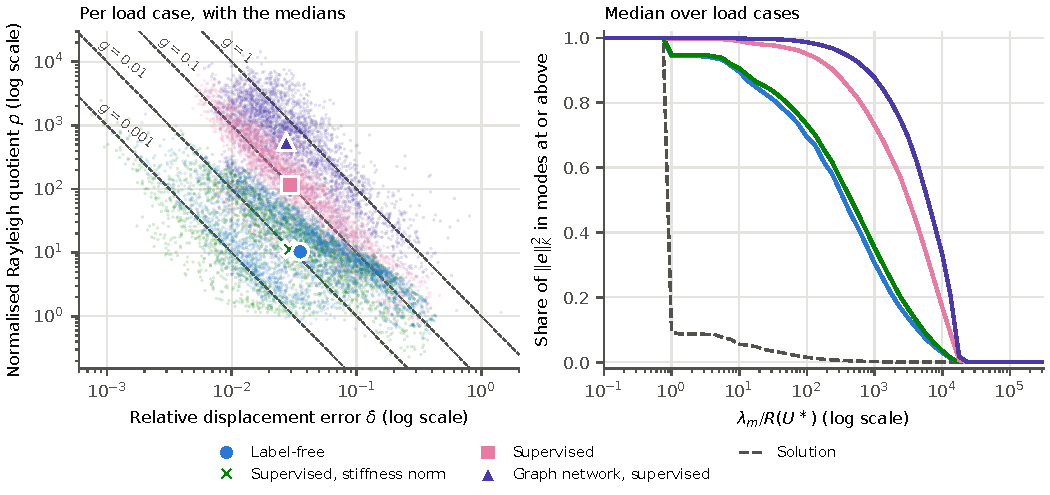
\includegraphics[width=\linewidth]{generated/fig_spectra.pdf}
\caption{Two dimensions, 1,024 labelled instances, measured after the run: where the errors
lie in the spectrum of the stiffness matrix. Left: for each of the \numSpecLoads{} triples
of seed, validation instance and load case (one point per triple and network), the
normalised Rayleigh quotient $\rho$ of the error against the relative displacement error
$\delta$ (\cref{rem:factor}); large markers are the medians of the two coordinates, and the
dashed lines are lines of equal relative energy gap $g=\rho\,\delta^2$. Right: for each
value of $\lambda_m/R(\Ustar)$ on the abscissa, the median over the triples of the share of
the error's squared stiffness norm in the eigenmodes at or above it; the dashed curve is the
same share of the solution's squared stiffness norm.}
\label{fig:spectra}
\end{figure}

The supervised and the stiffness-norm transformers, which differ only in the norm of the
loss, had errors of about the same size in different places. Over the triples, the geometric
mean of the ratio of their $\rho$, supervised over stiffness-norm, was \numSpecLabKnormRq{}
(\numSpecLabKnormRqSeeds{} in seeds 0, 1 and 2), and the supervised transformer's $\rho$ was
the larger on \numSpecLabKnormAbove{} of the triples. When each network's $\rho$ is first
averaged geometrically over its three seeds, which does not pair the seeds of the two
networks, the supervised transformer's was the larger on \numSpecLabKnormAboveSeedGm{} of
the \numSpecLoadCases{} pairs of instance and load case. The geometric mean of the ratio of
their $\delta^2$ was \numSpecLabKnormDisp{} (\numSpecLabKnormDispSeeds{}), and the
supervised transformer's $\delta$ was the smaller on \numSpecLabKnormDispLower{} of the
triples.

By \eqref{eq:factor}, the geometric mean of the ratio of their relative energy gaps,
\numSpecLabKnormGap{}, is the product of the two. On a logarithmic scale the ratio of $\rho$
accounts for \numSpecSpectralShare{} of it and the ratio of $\delta^2$ for the rest
(\numSpecSpectralShareMin{} to \numSpecSpectralShareMax{} in the three seeds; in the seed in
which the supervised transformer's errors were the smaller, the ratio of $\rho$ accounts for
more than the whole). This geometric mean is not the ratio of the seed means that H2a
tested, \numCmLabOverKnormGap{}, which the largest errors dominate. The modes with
$\lambda_m\ge 100\,R(\Ustar)$ held a median \numSpecShareKLab{} of the squared stiffness norm
of the supervised transformer's error, against \numSpecShareKKnorm{} for the stiffness-norm
transformer, \numSpecShareKFree{} for the label-free transformer and \numSpecShareKStar{} of
the solution's own.

The graph network's errors had the size of the supervised transformer's (ratio of
$\delta^2$, graph network over supervised, \numSpecMgnLabDisp{}) and lay higher still (ratio
of $\rho$ \numSpecMgnLabRq{}). The stiffness-norm and the label-free transformers, trained in
the same norm, had errors at the same place in the spectrum (ratio of $\rho$, stiffness-norm
over label-free, \numSpecKnormFreeRq{}) and of different sizes (ratio of $\delta^2$
\numSpecKnormFreeDisp{}; \numSpecKnormFreeDispSeeds{} in the three seeds): the
stiffness-norm transformer's errors were the smaller in every seed, by far the smaller in
seed 1, the seed that makes most of the difference in H3 (\cref{sec:results2d:norm}).

\begin{figure}[tbp]
\centering
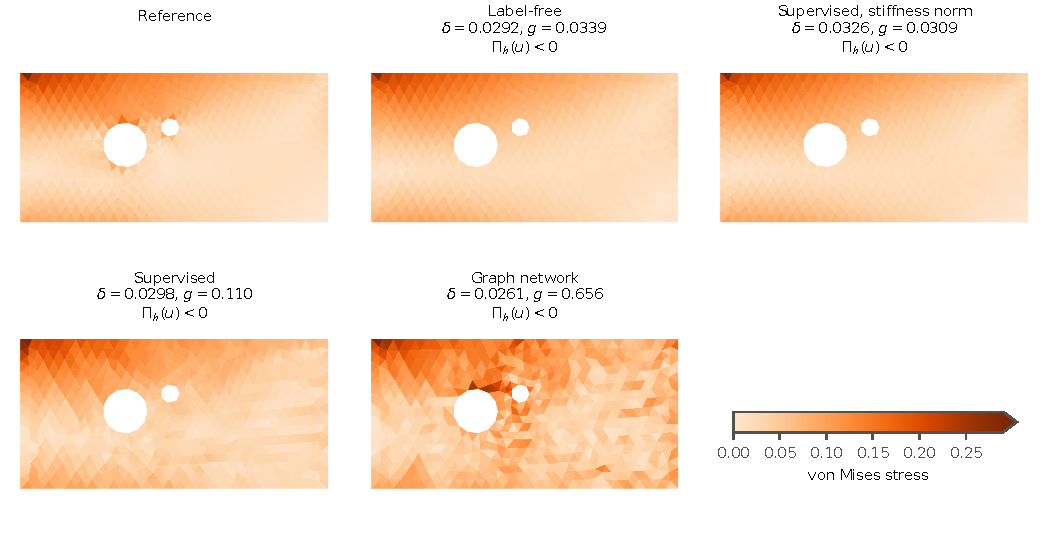
\includegraphics[width=\linewidth]{generated/fig_field2d.pdf}
\caption{Two dimensions, validation instance No.~\numSpecFigIndex{}, the one with the median
relative energy gap of the supervised transformer, seed 0, under the \numFigTwoDLoad{}
(selection rules in \cref{sec:methods:prereg}). Von Mises stress of the reference solution
and of the four networks with 1,024 labelled instances, on one colour scale set by the
reference. First row: the reference, then the two networks trained in the stiffness norm
(the label-free and the stiffness-norm transformers); second row: the two trained on the
displacement error (the supervised transformer and the graph network). Above each network,
its relative displacement error $\delta$ and relative energy gap $g$ on this load case and
the sign of $\Pi_h(u)$.}
\label{fig:field2d}
\end{figure}

\Cref{fig:field2d} shows one instance, chosen by the rule of \cref{sec:methods:prereg}
before the run's spectra were exported, in the load case that the same rule picks among its
four. On that load case, the four networks' displacement errors lay between
\numFigTwoDDispMin{} and \numFigTwoDDispMax{} and their relative energy gaps between
\numFigTwoDGapMin{} and \numFigTwoDGapMax{}; the stress fields of the two networks trained on
the displacement error are visibly rougher.

The networks ran with TF32 matrix products (\cref{sec:methods:training}), whose rounding
varies from node to node and therefore weighs heavily in the energy norm, so each network was
also evaluated with TF32 off. The rounding, the difference between the two predictions, had
a squared stiffness norm of a median \numSpecTfFree{} and \numSpecTfKnorm{} of that of the
error for the label-free and the stiffness-norm transformers (\numSpecTfLab{} and
\numSpecTfMgn{} for the two networks trained on the displacement error). In the modes with
$\lambda_m\ge10^4R(\Ustar)$ it had a median \numSpecTfStiffFree{} and
\numSpecTfStiffKnorm{} of the error's squared stiffness norm in those modes, on the
\numSpecTfStiffN{} triples whose spectra reach that far (\numSpecTfStiffLoads{} of the
\numSpecLoadCases{} pairs of instance and load case, in each seed). With TF32 off, the
median quotients $\rho$ were \numSpecIeeeRqFree{} (label-free), \numSpecIeeeRqKnorm{}
(stiffness norm), \numSpecIeeeRqLab{} (supervised) and \numSpecIeeeRqMgn{} (graph network),
and the geometric-mean ratios of $\rho$ and of $g$ between the supervised and the
stiffness-norm transformers rose to \numSpecIeeeLabKnormRq{} and \numSpecIeeeLabKnormGap{}.
The rounding thus places the errors of the two networks trained in the stiffness norm higher
in the spectrum than they would lie without it, and the readings as run understate the
differences between the networks trained in the two norms.

\subsection{Label efficiency}\label{sec:results2d:labels}

% generated by scripts/make_cmame_material.py from the records; do not edit
\begin{table}[tbp]
\centering
\footnotesize
\setlength{\tabcolsep}{4pt}
\caption{Label efficiency: relative displacement error / relative energy gap against the number of labelled training instances (seed means).}
\label{tab:labeleff}
\resizebox{\ifdim\width>\textwidth\textwidth\else\width\fi}{!}{%
\begin{tabular}{llcccc}
\toprule
Run & Model & 16 & 64 & 256 & 1,024 \\
\midrule
2D & Supervised & 0.459 / 20.8 & 0.165 / 3.06 & 0.0712 / 0.430 & 0.0505 / 0.133 \\
2D & Supervised, stiffness norm & 0.362 / 0.254 & 0.0889 / 0.0505 & 0.0667 / 0.0383 & 0.0547 / 0.0290 \\
2D & Graph network, supervised & -- & 0.370 / 149 & -- & 0.0499 / 0.825 \\
2D & Nearest-neighbour field & 0.687 / 6.50 & 0.466 / 1.65 & 0.408 / 1.03 & 0.404 / 0.959 \\
2D & Label-free (no labels) & 0.0634 / 0.0383 & 0.0634 / 0.0383 & 0.0634 / 0.0383 & 0.0634 / 0.0383 \\
\midrule
2D, July & Supervised & 0.272 / 6.26 & 0.193 / 2.72 & 0.176 / 1.26 & 0.160 / 0.418 \\
2D, July & Supervised + energy term & 0.410 / 2.56 & 0.184 / 0.579 & 0.182 / 0.154 & 0.161 / 0.166 \\
2D, July & Label-free, then supervised & 0.207 / 1.32 & 0.189 / 0.201 & 0.181 / 0.302 & 0.166 / 0.236 \\
2D, July & Graph network, supervised & 0.684 / 92.6 & 0.425 / 80.6 & 0.181 / 7.55 & 0.167 / 2.57 \\
2D, July & Label-free (no labels) & 0.166 / 0.0817 & 0.166 / 0.0817 & 0.166 / 0.0817 & 0.166 / 0.0817 \\
\midrule
3D & Supervised & 0.395 / 18.5 & 0.288 / 5.95 & 0.0726 / 0.799 & 0.0470 / 31.2 \\
3D & Supervised + energy term & 0.369 / 0.621 & 0.256 / 0.854 & 0.0833 / 0.964 & 0.0470 / 0.116 \\
3D & Graph network, supervised & -- & 0.149 / 18.3 & -- & 0.0168 / 0.447 \\
3D & Nearest-neighbour field & 0.648 / 5.74 & 0.477 / 2.24 & 0.400 / 1.20 & 0.382 / 1.22 \\
3D & Label-free (no labels) & 0.0300 / 0.00912 & 0.0300 / 0.00912 & 0.0300 / 0.00912 & 0.0300 / 0.00912 \\
\bottomrule
\end{tabular}}

\smallskip
\begin{minipage}{\linewidth}\footnotesize\raggedright
Seed means over 3 seeds (the nearest-neighbour field is deterministic, and the same in both 2D runs). A dash marks a budget at which the model was not trained (the graph network was trained at 64 and 1,024 labels only, except in the 2D run of July 2026). 2D: the run of 9 October 2026 (\cref{tab:2d}); 2D, July: the run of 16 July 2026, with the earlier code (\cref{tab:2djuly}). The label-free row repeats its single value, which uses the same 1,024 instances without labels.
\end{minipage}
\end{table}


\begin{figure}[tbp]
\centering
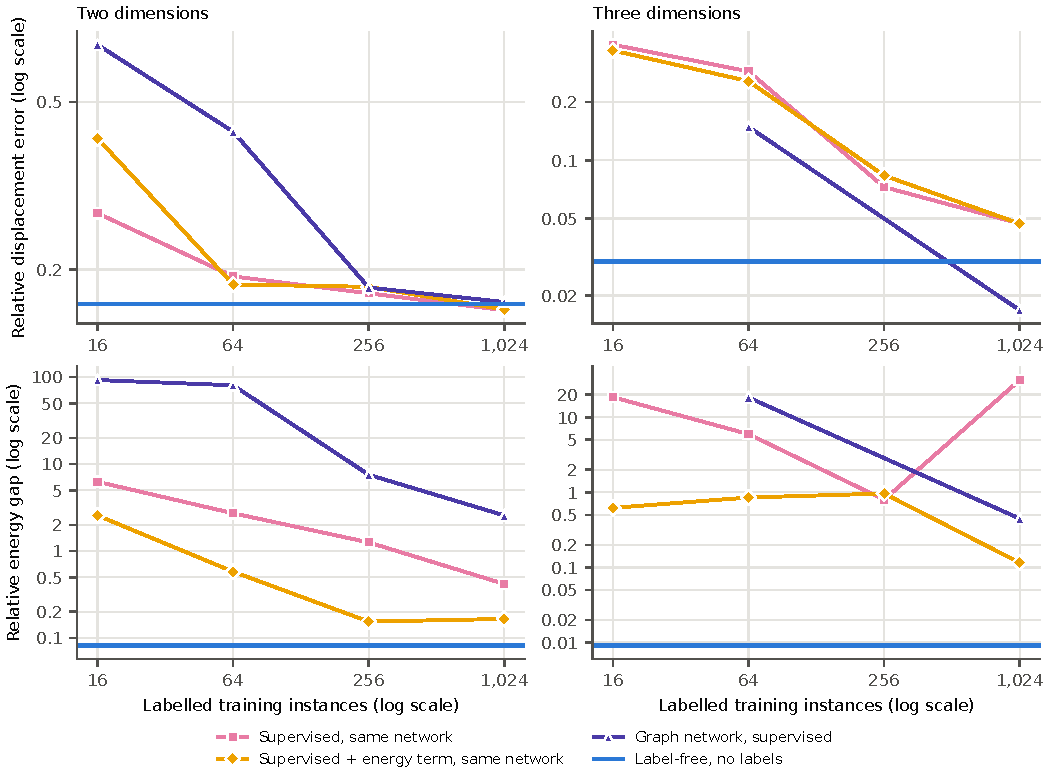
\includegraphics[width=\linewidth]{generated/fig_label_efficiency.pdf}
\caption{Label efficiency in two dimensions (left; the run of 9 October 2026) and three
dimensions (right): seed-mean relative displacement error (top) and relative energy gap
(bottom) of the supervised networks against the number of labelled training instances. The
horizontal line is the label-free transformer, trained on the same 1,024 instances without
their solutions. The stiffness-norm transformer was trained in two dimensions only, and the
graph network, in both panels, with 64 and 1,024 labels only; the supervised transformer
with the energy term is shown in three dimensions only (its two-dimensional values, from
the run of 16 July 2026, are in \cref{tab:labeleff}).}
\label{fig:labeleff}
\end{figure}

\Cref{tab:labeleff} and \cref{fig:labeleff} give the errors of the supervised networks
against the number of labelled instances. With no labels, the label-free transformer's
relative energy gap was lower than the supervised transformer's and the graph network's at
every budget; its advantage over the supervised transformer,
$1-g_{\text{label-free}}/g_{\text{supervised}}$ for the seed means, fell from
\numCmAdvMax{} with 16 labels to \numCmAdvMin{} with 1,024. In displacement, the supervised
transformer and the graph network needed 1,024 labels to pass it.

The pre-registration also compared the supervised and the stiffness-norm transformers with
the label-free transformer on every metric at every budget, by the same guard, as readings
without verdicts. These are among its \numCmSecondary{} secondary readings, which are
exploratory and not corrected for multiplicity, so that some crossings of the guard are
expected by chance. The supervised transformer was worse than the label-free transformer
beyond the guard in relative energy gap, von Mises error, peak stress error and
critical-region recall at every budget. The stiffness-norm transformer was worse beyond the
guard on every metric with 16 labelled instances and on every metric but the
critical-region recall with 64, and within the guard on every metric with 256 and 1,024;
its seed means fell below the label-free transformer's, in relative energy gap and in
displacement, with 1,024 labels only. With 16, 64 and 256 labelled instances,
\numCmLabWorseSixteen{}, \numCmLabWorseSixtyFour{} and \numCmLabWorseTwoFiveSix{} of the
supervised transformer's \numCmPairs{} instance-seed predictions were worse than the zero
field, against \numCmKnormWorseSixteen{}, \numCmKnormWorseSixtyFour{} and
\numCmKnormWorseTwoFiveSix{} for the stiffness-norm transformer. Supervised in the stiffness
norm, 256 labelled instances brought the transformer's seed means within the guard of the
label-free transformer's on every metric, although the label-free transformer still had the
lower relative energy gap on \numPairCmFreeKnormGapTwoFiveSix{} of the instance-seed pairs;
supervised on the displacement error, 1,024 left a von Mises error \numCmLabOverFreeVm{}
times the label-free transformer's.

\subsection{The run of 16 July 2026}\label{sec:results2d:july}

The run of 16 July 2026, pre-registered before it was executed, compared the networks on the
same corpus, split and seeds with the code of July 2026, in which the decoder did not
multiply $F_{\max}$ back onto the prediction, so that no network in that run could know the
absolute amplitude of an instance's loads (\cref{sec:methods:networks}). It also trained
what the run of 9 October 2026 did not: the supervised transformer with an energy term, the
supervised transformer trained from the label-free transformer's parameters
(\cref{sec:methods:training}), and the graph network with every number of labelled
instances. It trained no stiffness-norm transformer.

\subsubsection{Accuracy and label efficiency}\label{sec:results2d:julyaccuracy}

% generated by scripts/make_cmame_material.py from the records; do not edit
\begin{table}[tbp]
\centering
\footnotesize
\setlength{\tabcolsep}{4pt}
\caption{Two-dimensional plates, the run of 16 July 2026 with the earlier code (\cref{sec:results2d:july}): every metric at the largest label budget, on the instances of \cref{tab:2d}.}
\label{tab:2djuly}
\resizebox{\ifdim\width>\textwidth\textwidth\else\width\fi}{!}{%
\begin{tabular}{lcccccc}
\toprule
Model & \shortstack{Displacement \\ error} & \shortstack{Relative \\ energy gap} & \shortstack{von Mises \\ error} & \shortstack{Peak stress \\ error} & \shortstack{Critical-region \\ recall} & \shortstack{Worse than \\ zero field} \\
\midrule
Label-free & 0.166 $\pm$ 0.002 & 0.0817 $\pm$ 0.0040 & 0.210 $\pm$ 0.003 & 0.228 $\pm$ 0.001 & 0.739 $\pm$ 0.003 & 3/768 \\
Supervised & 0.160 $\pm$ 0.003 & 0.418 $\pm$ 0.037 & 0.433 $\pm$ 0.031 & 0.334 $\pm$ 0.036 & 0.584 $\pm$ 0.027 & 52/768 \\
Supervised + energy term & 0.161 $\pm$ 0.005 & 0.166 $\pm$ 0.040 & 0.257 $\pm$ 0.007 & 0.246 $\pm$ 0.022 & 0.708 $\pm$ 0.012 & 14/768 \\
Label-free, then supervised & 0.166 $\pm$ 0.006 & 0.236 $\pm$ 0.032 & 0.336 $\pm$ 0.020 & 0.301 $\pm$ 0.019 & 0.645 $\pm$ 0.008 & 21/768 \\
Graph network, supervised & 0.167 $\pm$ 0.000 & 2.57 $\pm$ 0.25 & 1.10 $\pm$ 0.07 & 1.32 $\pm$ 0.13 & 0.322 $\pm$ 0.027 & 481/768 \\
\midrule
Nearest-neighbour field & 0.404 & 0.959 & 0.735 & 0.643 & 0.515 & 94/256 \\
Scaled polynomial & 1.42 & 873 & 11.4 & 30.8 & 0.159 & 256/256 \\
\midrule
Zero field & 1.00 & 1.00 & 1.00 & 1.00 & -- & -- \\
\bottomrule
\end{tabular}}

\smallskip
\begin{minipage}{\linewidth}\footnotesize\raggedright
256 validation instances, never trained on; four load cases each. Errors are relative to the reference finite-element solution, per load case, then averaged over the load cases; the relative energy gap of the zero field is 1. Trained networks: mean $\pm$ sample standard deviation over 3 seeds; the nearest-neighbour field and the scaled polynomial are deterministic.\par
Worse than zero field: instance-seed pairs whose relative energy gap exceeds 1, that is, predictions further from the solution in the energy norm than the zero field.\par
Critical-region recall: the share of the 10\% most stressed elements of the reference solution that are also among the 10\% most stressed of the prediction (higher is better; in every other column lower is better).\par
Run of 16 July 2026. Its code did not multiply the load scale back onto the output (\cref{sec:methods:networks}); we attribute the narrow spread of the displacement errors to this; no experiment isolated it (\cref{sec:results2d:julyaccuracy}).
\end{minipage}
\end{table}


\Cref{tab:2djuly} gives every metric with 1,024 labelled instances. The supervised
transformer had the lowest displacement error, \numTwoLabDispFour{} against
\numTwoFreeDispFour{} for the label-free transformer, which was \numTwoFreeDispExcessAbs{}
higher, and higher in each of the three seeds. On every other metric the label-free
transformer was the most accurate network in the table: its relative energy gap,
\numTwoFreeGap{}, was \numTwoLabOverFreeGap{} times lower than the supervised transformer's,
and its von Mises error (\numTwoFreeVm{} against \numTwoLabVm{}), peak stress error
(\numTwoFreePeak{} against \numTwoLabPeak{}) and critical-region recall (\numTwoFreeRecall{}
against \numTwoLabRecall{}) were better. Compared instance by instance within each seed, the
label-free transformer had the lower relative energy gap on \numPairTwoLabGap{} of the
\numTwoPairs{} instance-seed pairs and the lower von Mises error on \numPairTwoLabVm{}, but
the lower displacement error on only \numPairTwoLabDisp{}. The energy term lowered the
supervised transformer's relative energy gap to \numTwoAncGap{} and its von Mises error to
\numTwoAncVm{}, both still above the label-free values. The graph network matched the others
in displacement (\numTwoMgnDisp{}) but had a relative energy gap of \numTwoMgnGap{} and a von
Mises error of \numTwoMgnVm{}: \numTwoMgnWorse{} of its \numTwoPairs{} instance-seed
predictions were further from the solution, in the energy norm, than the zero field. The
supervised transformer had \numTwoLabWorse{} such predictions, the supervised transformer
with the energy term \numTwoAncWorse{}, and the label-free transformer \numTwoFreeWorse{},
one per seed.

The displacement errors of the five trained networks lie between \numTwoLabDisp{} and
\numTwoMgnDisp{}, a narrow band, while their relative energy gaps span a factor of
\numTwoGapSpread{}. We attribute the narrow band to the code: no network could know the
absolute amplitude of an instance's loads, which adds an error common to every displacement
and compresses their differences. With the later code, the displacement errors of the
label-free transformer, the supervised transformer and the graph network on the same
instances were \numJulyOverCmDispMin{} to \numJulyOverCmDispMax{} times lower
(\cref{tab:2d}), and those of the trained networks spanned a factor of \numCmDispSpread{}
rather than \numTwoDispSpread{}. This agrees with the attribution, but the two runs also
differ in their software versions, and no experiment isolated the output scaling.

With no labels, the label-free transformer's relative energy gap was lower than every
supervised network's at every budget (\cref{tab:labeleff}); its advantage over the supervised
transformer fell from \numTwoAdvMax{} with 16 labels to \numTwoAdvMin{} with 1,024. In
displacement, the supervised transformer needed 1,024 labels to pass it. With 16 labels, the
supervised transformer with the energy term was less accurate in displacement than without
it, and its per-seed errors scattered widely (\numTwoAncSixteenSeeds{}); an exploratory run
later traced this to the instability of the gradient-scaled energy term with very few labels
(\ref{app:prereg}). With 16 labels the supervised transformer of the later code was less
accurate than that of July 2026, with a relative energy gap of \numCmLabGapSixteen{} against
\numTwoLabGapSixteen{}.

\subsubsection{Pre-registered decisions}\label{sec:results2d:decisions}

The gate of this run concerned the energy term and pretraining rather than the label-free
network alone, and all three of its conditions were met (\cref{tab:criteria}). Its first
condition read a separate energy-term sub-experiment of the same run, which trained its own
supervised transformers with and without the energy term in the same configuration: there,
the supervised transformer with the energy term was \numGOneSanityMin{} to
\numGOneSanityMax{} times more accurate in displacement than the zero field and beat the two
naive baselines and the plain polynomial (\cref{sec:methods:networks}), all fitted on 1,024
labelled instances, at every budget. The other two conditions read the networks of
\cref{tab:2djuly,tab:labeleff}: with 64 labels, the energy term lowered the relative energy
gap by \numGOneGapReduction{} and the von Mises error by \numGOneVmReduction{}, and
label-free training followed by supervised training beat supervised training alone by
\numGOneFtGap{} in relative energy gap. The kill conditions on the label-free network were not
triggered: its displacement error was within the 30\% allowed by K2, and its relative
energy-gap advantage stayed above the 40\% floor at every budget. Two kill conditions were
triggered, and both claims were withdrawn.

\paragraph{Warm start (K5)}
On \numKfiveEval{} validation instances and four load cases each, unpreconditioned
conjugate gradients needed on average \numKfiveZero{} iterations from the zero field to
reach a relative residual of \numKfiveTol{}, \numKfiveFree{} from the prediction of a
label-free transformer (trained for 100 epochs for this test) and \numKfiveNaive{} from
the scaled polynomial: savings of \numKfiveSaving{} and \numKfiveNaiveSaving{} against the
20\% required. The prediction was accurate in energy, $g=\numKfiveStartGap{}$, and five
and twenty iterations from it lowered the relative energy gap to \numKfiveFiveGap{} and
\numKfiveTwentyGap{}, but it did not shorten the run to the tolerance. This is consistent
with \cref{cor:warm,rem:residual}: at a tight tolerance a warm start of this accuracy lowers
the iteration bound by only a small fraction, and a residual-based stop can see a
prediction accurate in energy as further from convergence than the zero field. Neither the
initial residuals nor energy-based stopping were measured, so the two effects cannot be
separated here.

\paragraph{Cross-resolution regulariser (K6)}
A term that penalised differences between the latent representations of the same instance
meshed at two resolutions did not shrink the transfer gap, the increase of the
displacement error from the training resolution to a finer one; it widened it, by
\numCoarsenHighWiden{} for meshes coarsened by a factor of \numCoarsenHigh{} and by
\numCoarsenLowWiden{} for \numCoarsenLow{}. The regulariser plays no further part in this
paper.

\subsubsection{Further observations}\label{sec:results2d:other}

\paragraph{Replication}
An exploratory run on 30 July 2026, which was not pre-registered, trained the label-free
transformer \numDiagSeeds{} more times with the same configuration, with seeds 0 to 5. The
first three repeat the seed numbers of the run of 16 July 2026 but did not reproduce its values
exactly; the replication ran on a different GPU model and a later release of the code whose
training path is unchanged. Over all \numTwoRuns{} trainings the displacement error was
\numTwoRunsDisp{} and the relative energy gap \numTwoRunsGap{} (mean and sample standard
deviation).

\paragraph{Cross-resolution transfer}
In the test of K6, label-free transformers trained for 100 epochs, with seed 0, on 512
coarsened meshes and without the regulariser were evaluated on the coarsened and on the
original meshes of 128 held-out instances. The displacement error rose from
\numCoarsenLowCoarse{} to \numCoarsenLowFine{} for meshes \numCoarsenLow{} times finer
than in training and from \numCoarsenHighCoarse{} to \numCoarsenHighFine{} for meshes
\numCoarsenHigh{} times finer. In this code version the output did not depend on the mesh
through $F_{\max}$; the contrast with three dimensions is taken up in \cref{sec:transfer}.
